\documentclass[tikz,border=6pt]{standalone}
\usepackage{amsmath}
\usepackage{newtxtext,newtxmath}
\usetikzlibrary{arrows.meta,calc,positioning,shapes.geometric}

\begin{document}
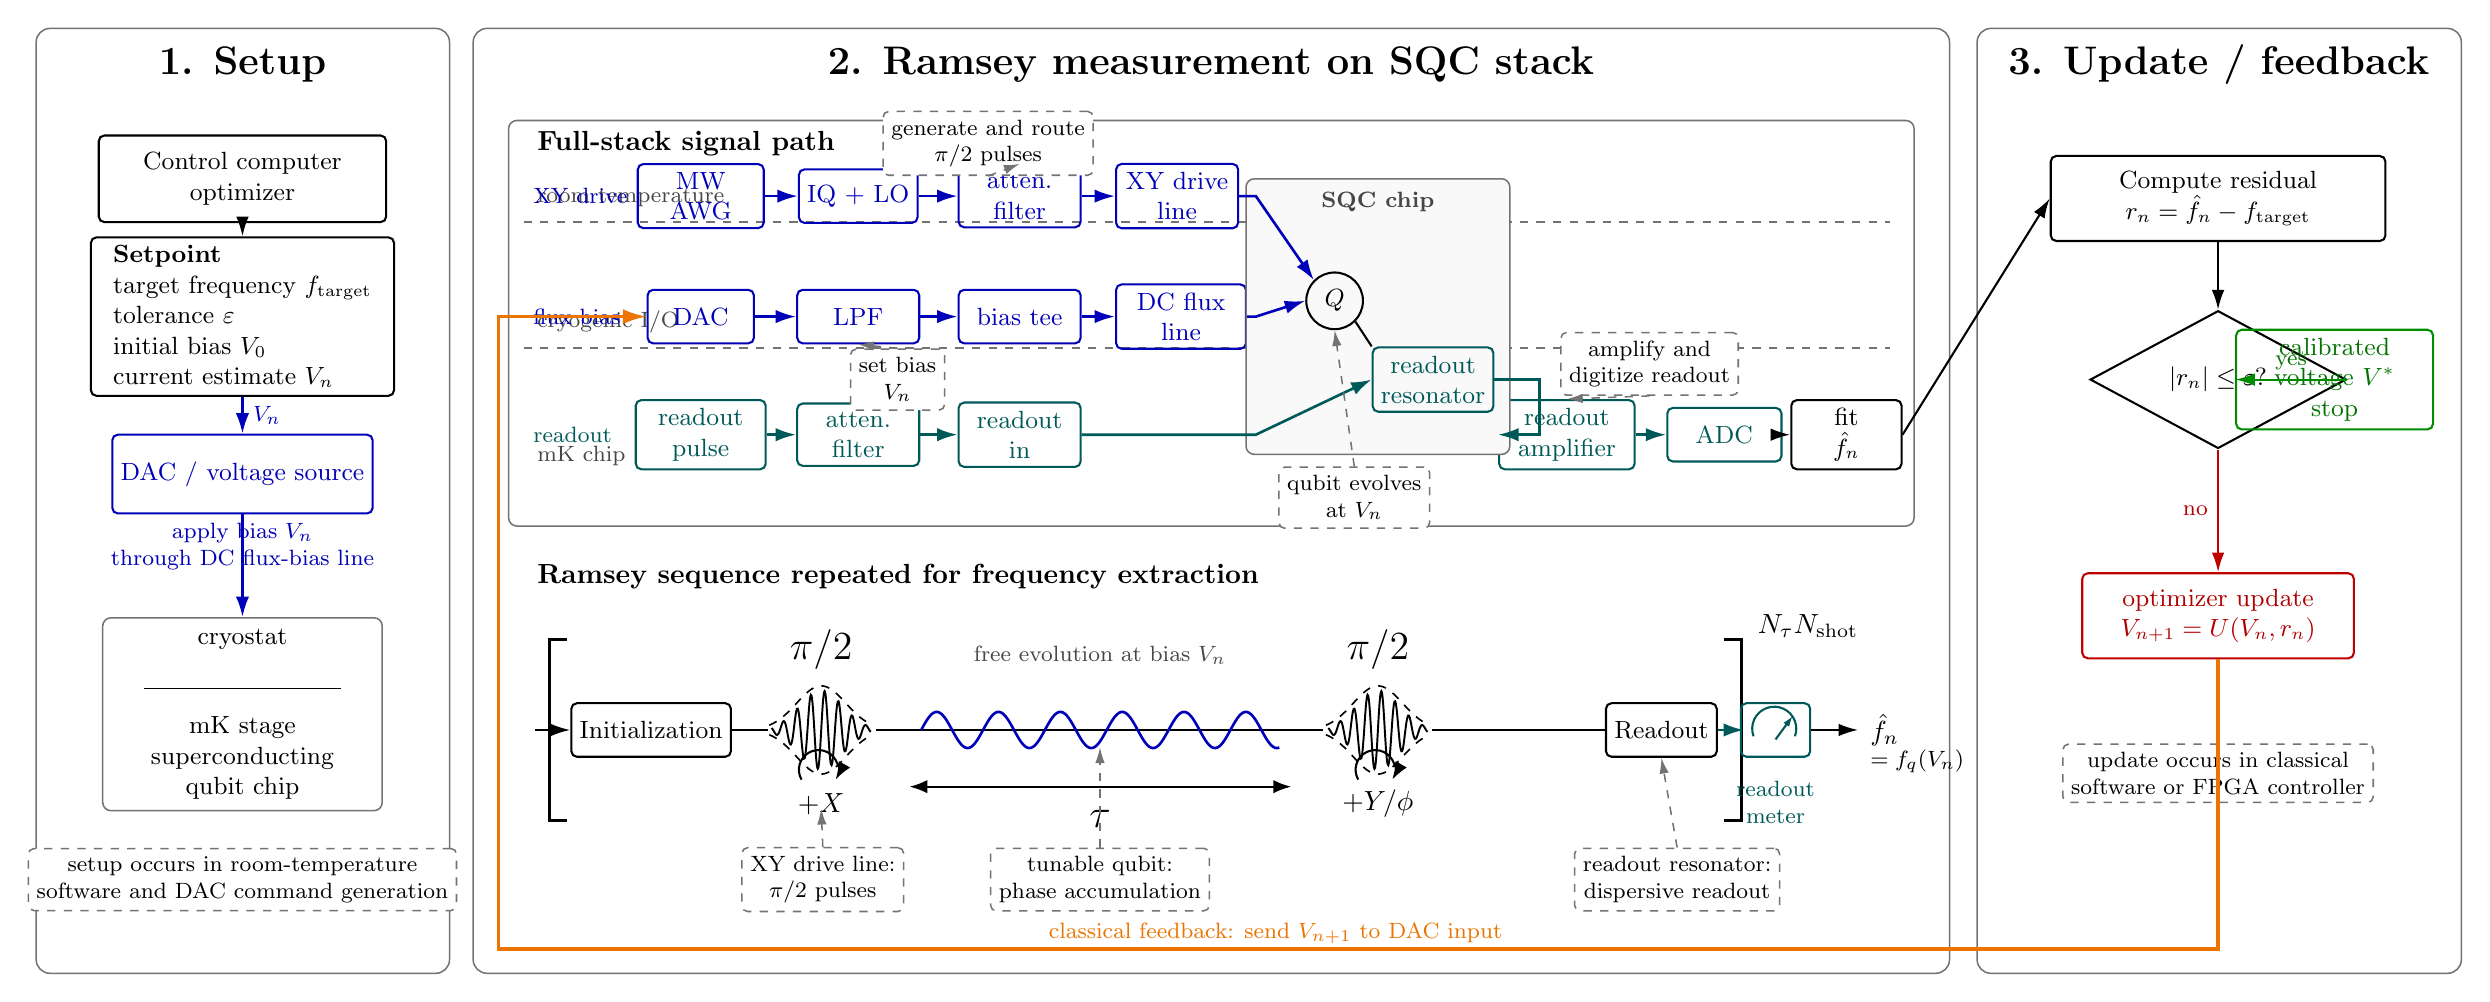
\begin{tikzpicture}[
  x=1cm,
  y=1cm,
  >=Latex,
  font=\small,
  line/.style={draw=black,line width=0.75pt},
  thinbox/.style={draw=black!55,line width=0.55pt},
  ctrl/.style={draw=blue!72!black,line width=0.95pt},
  read/.style={draw=teal!70!black,line width=0.95pt},
  feed/.style={draw=orange!92!black,line width=1.2pt},
  arrow/.style={line,-{Latex[length=2.5mm,width=1.6mm]}},
  ctrlarrow/.style={ctrl,-{Latex[length=2.6mm,width=1.7mm]}},
  readarrow/.style={read,-{Latex[length=2.6mm,width=1.7mm]}},
  feedarrow/.style={feed,-{Latex[length=3.0mm,width=1.9mm]}},
  panel/.style={thinbox,rounded corners=5pt,fill=white},
  block/.style={line,rounded corners=2pt,align=center,inner sep=3pt,minimum height=0.68cm},
  blueblock/.style={block,draw=blue!72!black,text=blue!72!black},
  tealblock/.style={block,draw=teal!70!black,text=teal!70!black},
  redblock/.style={block,draw=red!75!black,text=red!70!black},
  greenblock/.style={block,draw=green!55!black,text=green!45!black},
  callout/.style={thinbox,dashed,rounded corners=2pt,align=center,fill=white,inner sep=3pt,font=\footnotesize},
  pulse/.style={draw=black,line width=0.70pt},
  env/.style={draw=black,dashed,line width=0.58pt},
  note/.style={font=\footnotesize,align=center,text=black!72},
  bluelabel/.style={font=\footnotesize,text=blue!72!black,align=center},
  teallabel/.style={font=\footnotesize,text=teal!70!black,align=center},
  orangelabel/.style={font=\footnotesize,text=orange!92!black,align=center}
]

% ---------------------------------------------------------------------------
% Main panels
\node[panel,minimum width=5.25cm,minimum height=12.0cm,anchor=south west] (Psetup) at (0,0) {};
\node[panel,minimum width=18.75cm,minimum height=12.0cm,anchor=south west] (Pmeas) at (5.55,0) {};
\node[panel,minimum width=6.15cm,minimum height=12.0cm,anchor=south west] (Pupd) at (24.65,0) {};

\node[font=\bfseries\Large] at (2.63,11.55) {1. Setup};
\node[font=\bfseries\Large] at (14.93,11.55) {2. Ramsey measurement on SQC stack};
\node[font=\bfseries\Large] at (27.73,11.55) {3. Update / feedback};

% ---------------------------------------------------------------------------
% Setup panel
\node[block,minimum width=3.65cm,minimum height=1.10cm] (setCPU) at (2.63,10.10)
  {Control computer\\optimizer};
\node[block,minimum width=3.85cm,minimum height=1.55cm,align=left] (setList) at (2.63,8.35)
  {\textbf{Setpoint}\\
   target frequency $f_{\mathrm{target}}$\\
   tolerance $\varepsilon$\\
   initial bias $V_0$\\
   current estimate $V_n$};
\node[blueblock,minimum width=3.05cm,minimum height=1.00cm] (setDAC) at (2.63,6.35)
  {DAC / voltage source};
\node[bluelabel] at (2.63,5.43) {apply bias $V_n$\\through DC flux-bias line};
\node[thinbox,rounded corners=3pt,minimum width=3.55cm,minimum height=2.45cm,align=center] (cryo) at (2.63,3.30)
  {cryostat\\[0.18cm]\rule{2.5cm}{0.25pt}\\[0.18cm]
   mK stage\\superconducting\\qubit chip};
\draw[arrow] (setCPU.south) -- (setList.north);
\draw[ctrlarrow] (setList.south) -- node[right,font=\footnotesize,text=blue!72!black] {$V_n$} (setDAC.north);
\draw[ctrlarrow] (setDAC.south) -- (cryo.north);

% Stage labels near setup.
\node[callout] at (2.63,1.20) {setup occurs in room-temperature\\software and DAC command generation};

% ---------------------------------------------------------------------------
% Full-stack SQC circuit map in the measurement panel
\node[thinbox,rounded corners=3pt,minimum width=17.85cm,minimum height=5.15cm,anchor=north west] (stackbox) at (6.00,10.85) {};
\node[anchor=west,font=\bfseries] at (6.25,10.55) {Full-stack signal path};
\draw[thinbox,dashed] (6.20,9.55) -- (23.55,9.55);
\draw[thinbox,dashed] (6.20,7.95) -- (23.55,7.95);
\node[anchor=west,note] at (6.25,9.86) {room temperature};
\node[anchor=west,note] at (6.25,8.28) {cryogenic I/O};
\node[anchor=west,note] at (6.25,6.58) {mK chip};

% Three separated lanes: drive, flux-bias, and readout.
\node[bluelabel,anchor=west] at (6.20,9.88) {XY drive};
\node[bluelabel,anchor=west] at (6.20,8.35) {flux bias};
\node[teallabel,anchor=west] at (6.20,6.85) {readout};

% XY drive lane
\node[blueblock,minimum width=1.60cm] (mw) at (8.45,9.88) {MW\\AWG};
\node[blueblock,minimum width=1.50cm] (iq) at (10.45,9.88) {IQ + LO};
\node[blueblock,minimum width=1.55cm] (xyChain) at (12.50,9.88) {atten.\\filter};
\node[blueblock,minimum width=1.55cm] (xyLine) at (14.50,9.88) {XY drive\\line};
\draw[ctrlarrow] (mw.east) -- (iq.west);
\draw[ctrlarrow] (iq.east) -- (xyChain.west);
\draw[ctrlarrow] (xyChain.east) -- (xyLine.west);

% Flux-bias lane
\node[blueblock,minimum width=1.35cm] (dac) at (8.45,8.35) {DAC};
\node[blueblock,minimum width=1.55cm] (fluxChain) at (10.45,8.35) {LPF};
\node[blueblock,minimum width=1.55cm] (biasTee) at (12.50,8.35) {bias tee};
\node[blueblock,minimum width=1.65cm] (fluxLine) at (14.55,8.35) {DC flux\\line};
\draw[ctrlarrow] (dac.east) -- (fluxChain.west);
\draw[ctrlarrow] (fluxChain.east) -- (biasTee.west);
\draw[ctrlarrow] (biasTee.east) -- (fluxLine.west);

% Readout lane: source to chip and return to digitizer.
\node[tealblock,minimum width=1.65cm] (roSrc) at (8.45,6.85) {readout\\pulse};
\node[tealblock,minimum width=1.55cm] (roInChain) at (10.45,6.85) {atten.\\filter};
\node[tealblock,minimum width=1.55cm] (roLineIn) at (12.50,6.85) {readout\\in};
\node[tealblock,minimum width=1.72cm] (amp) at (19.45,6.85) {readout\\amplifier};
\node[tealblock,minimum width=1.45cm] (adc) at (21.45,6.85) {ADC};
\node[block,minimum width=1.40cm] (fit) at (23.00,6.85) {fit\\$\hat f_n$};
\draw[readarrow] (roSrc.east) -- (roInChain.west);
\draw[readarrow] (roInChain.east) -- (roLineIn.west);

% Chip is separated on the right, with clean vertical entry points.
\node[thinbox,rounded corners=3pt,fill=gray!5,minimum width=3.35cm,minimum height=3.50cm] (chipbox) at (17.05,8.35) {};
\node[note,font=\footnotesize\bfseries] at (17.05,9.80) {SQC chip};
\node[circle,line,minimum size=0.72cm] (qubit) at (16.50,8.55) {$Q$};
\node[tealblock,minimum width=1.35cm,minimum height=0.52cm] (res) at (17.75,7.55) {readout\\resonator};
\draw[line] (qubit.south east) -- (res.north west);
\coordinate (xyPort) at (15.50,9.88);
\coordinate (fluxPort) at (15.50,8.35);
\coordinate (roInPort) at (15.50,6.85);
\coordinate (roOutPort) at (18.65,7.55);
\draw[ctrlarrow] (xyLine.east) -- (xyPort) -- (qubit.north west);
\draw[ctrlarrow] (fluxLine.east) -- (fluxPort) -- (qubit.west);
\draw[readarrow] (roLineIn.east) -- (roInPort) -- (res.west);
\draw[readarrow] (res.east) -- (roOutPort) -- ++(0.45,0) |- (amp.west);
\draw[readarrow] (amp.east) -- (adc.west);
\draw[arrow] (adc.east) -- (fit.west);

% Operation callouts placed in empty space, not on top of the lines.
\node[callout] (opPulse) at (12.10,10.55) {generate and route\\$\pi/2$ pulses};
\node[callout] (opBias) at (10.95,7.55) {set bias\\$V_n$};
\node[callout] (opEvolve) at (16.75,6.05) {qubit evolves\\at $V_n$};
\node[callout] (opRead) at (20.50,7.75) {amplify and\\digitize readout};
\draw[thinbox,dashed,-{Latex[length=2.0mm,width=1.2mm]}] (opPulse.south) -- (xyChain.north);
\draw[thinbox,dashed,-{Latex[length=2.0mm,width=1.2mm]}] (opBias.north) -- (fluxChain.south);
\draw[thinbox,dashed,-{Latex[length=2.0mm,width=1.2mm]}] (opEvolve.north) -- (qubit.south);
\draw[thinbox,dashed,-{Latex[length=2.0mm,width=1.2mm]}] (opRead.south) -- (amp.north);

% ---------------------------------------------------------------------------
% Ramsey pulse sequence in the measurement panel
\node[anchor=west,font=\bfseries] at (6.25,5.05) {Ramsey sequence repeated for frequency extraction};
\coordinate (seqL) at (6.75,3.10);
\coordinate (seqR) at (21.45,3.10);
\draw[line width=1.0pt] ($(seqL)+(0,1.15)$) -- ++(-0.22,0) -- ++(0,-2.30) -- ++(0.22,0);
\draw[line width=1.0pt] ($(seqR)+(0,1.15)$) -- ++(0.22,0) -- ++(0,-2.30) -- ++(-0.22,0);
\node[anchor=south west,font=\normalsize] at ($(seqR)+(0.30,1.05)$) {$N_\tau N_{\mathrm{shot}}$};

\node[block,minimum width=1.65cm] (init) at (7.82,3.10) {Initialization};
\node[block,minimum width=1.25cm] (readout) at (20.65,3.10) {Readout};
\draw[arrow] (6.35,3.10) -- (init.west);
\draw[line] (init.east) -- (9.30,3.10);
\draw[line] (10.68,3.10) -- (16.35,3.10);
\draw[line] (17.74,3.10) -- (readout.west);
\draw[readarrow] (readout.east) -- (21.70,3.10);

% First pi/2 pulse
\begin{scope}[shift={(9.98,3.10)}]
  \node[font=\Large] at (0,1.02) {$\pi/2$};
  \draw[pulse,domain=-0.63:0.63,samples=130,smooth]
    plot (\x,{0.50*exp(-6.5*\x*\x)*sin(deg(36*\x))});
  \draw[env,domain=-0.66:0.66,samples=80,smooth]
    plot (\x,{0.56*exp(-5.1*\x*\x)});
  \draw[env,domain=-0.66:0.66,samples=80,smooth]
    plot (\x,{-0.56*exp(-5.1*\x*\x)});
  \draw[->,line width=0.75pt] (-0.25,-0.63) arc[start angle=210,end angle=-30,radius=0.25];
  \node[font=\normalsize] at (0,-0.94) {$+X$};
\end{scope}

% Second pi/2 pulse
\begin{scope}[shift={(17.05,3.10)}]
  \node[font=\Large] at (0,1.02) {$\pi/2$};
  \draw[pulse,domain=-0.63:0.63,samples=130,smooth]
    plot (\x,{0.50*exp(-6.5*\x*\x)*sin(deg(36*\x))});
  \draw[env,domain=-0.66:0.66,samples=80,smooth]
    plot (\x,{0.56*exp(-5.1*\x*\x)});
  \draw[env,domain=-0.66:0.66,samples=80,smooth]
    plot (\x,{-0.56*exp(-5.1*\x*\x)});
  \draw[->,line width=0.75pt] (-0.25,-0.63) arc[start angle=210,end angle=-30,radius=0.25];
  \node[font=\normalsize] at (0,-0.94) {$+Y/\phi$};
\end{scope}

% Free evolution interval and phase oscillation
\draw[Latex-Latex,line width=0.78pt] (11.10,2.38) -- (15.95,2.38);
\node[font=\Large] at (13.52,1.97) {$\tau$};
\draw[ctrl,domain=11.25:15.80,samples=180,smooth]
  plot (\x,{3.10 + 0.23*sin(deg(8.0*(\x-11.25)))});
\node[note] at (13.52,4.05) {free evolution at bias $V_n$};

% Instrument-style readout meter
\node[tealblock,minimum width=0.88cm,minimum height=0.68cm] (meter) at (22.10,3.10) {};
\draw[read,line width=0.75pt] (21.82,3.02) arc[start angle=200,end angle=-20,radius=0.28];
\draw[read,-{Latex[length=1.4mm,width=0.9mm]},line width=0.75pt] (22.10,2.98) -- (22.32,3.28);
\node[teallabel,anchor=north] at (22.10,2.57) {readout\\meter};
\draw[arrow] (22.55,3.10) -- (23.15,3.10);
\node[anchor=west,font=\normalsize] (fhat) at (23.18,3.10) {$\hat f_n$};
\node[anchor=west,font=\footnotesize] at (23.18,2.70) {$=f_q(V_n)$};

% Operation labels attached to the Ramsey sequence
\node[callout] (seqDrive) at (10.00,1.20) {XY drive line:\\$\pi/2$ pulses};
\node[callout] (seqQ) at (13.52,1.20) {tunable qubit:\\phase accumulation};
\node[callout] (seqRead) at (20.85,1.20) {readout resonator:\\dispersive readout};
\draw[thinbox,dashed,-{Latex[length=2.0mm,width=1.2mm]}] (seqDrive.north) -- (9.98,2.10);
\draw[thinbox,dashed,-{Latex[length=2.0mm,width=1.2mm]}] (seqQ.north) -- (13.52,2.88);
\draw[thinbox,dashed,-{Latex[length=2.0mm,width=1.2mm]}] (seqRead.north) -- (readout.south);

% ---------------------------------------------------------------------------
% Update and feedback panel
\node[block,minimum width=4.25cm,minimum height=1.08cm] (resid) at (27.72,9.85)
  {Compute residual\\$r_n=\hat f_n-f_{\mathrm{target}}$};
\node[diamond,line,aspect=1.90,inner sep=1.5pt,minimum width=3.25cm,minimum height=1.75cm,align=center] (decide) at (27.72,7.55)
  {$|r_n|\leq \varepsilon$?};
\node[greenblock,minimum width=2.50cm,minimum height=1.10cm] (done) at (29.20,7.55)
  {calibrated\\voltage $V^\ast$\\stop};
\node[redblock,minimum width=3.45cm,minimum height=1.08cm] (upd) at (27.72,4.55)
  {optimizer update\\$V_{n+1}=U(V_n,r_n)$};
\node[callout] at (27.72,2.55) {update occurs in classical\\software or FPGA controller};
\draw[arrow] (resid.south) -- (decide.north);
\draw[arrow,draw=green!55!black] (decide.east) -- node[above,font=\footnotesize,text=green!45!black] {yes} (done.west);
\draw[arrow,draw=red!75!black] (decide.south) -- node[left,font=\footnotesize,text=red!70!black] {no} (upd.north);
\draw[arrow] (fit.east) -- (resid.west);

% Classical feedback loop routed below all active content and terminating at DAC.
\draw[feedarrow] (upd.south) -- (27.72,0.32) -- (5.88,0.32) -- (5.88,8.35) -- (dac.west);
\node[orangelabel,fill=white,inner sep=1pt] at (15.75,0.52) {classical feedback: send $V_{n+1}$ to DAC input};

\end{tikzpicture}
\end{document}
